% \iffalse
\let\negmedspace\undefined
\let\negthickspace\undefined
\documentclass[journal,12pt,twocolumn]{IEEEtran}
\usepackage{cite}
\usepackage{amsmath,amssymb,amsfonts,amsthm}
\usepackage{algorithmic}
\usepackage{graphicx}
\usepackage{textcomp}
\usepackage{xcolor}
\usepackage{txfonts}
\usepackage{listings}
\usepackage{enumitem}
\usepackage{mathtools}
\usepackage{gensymb}
\usepackage{comment}
\usepackage[breaklinks=true]{hyperref}
\usepackage{tkz-euclide} 
\usepackage{listings}
\usepackage{gvv}                                        
\def\inputGnumericTable{}                                 
\usepackage[latin1]{inputenc}                                
\usepackage{color}                                            
\usepackage{array}                                            
\usepackage{longtable}                                       
\usepackage{calc}                                             
\usepackage{multirow}                                         
\usepackage{hhline}                                           
\usepackage{ifthen}                                           
\usepackage{lscape}
\usepackage{placeins}
\usepackage{xparse}


\newtheorem{theorem}{Theorem}[section]
\newtheorem{problem}{Problem}
\newtheorem{proposition}{Proposition}[section]
\newtheorem{lemma}{Lemma}[section]
\newtheorem{corollary}[theorem]{Corollary}
\newtheorem{example}{Example}[section]
\newtheorem{definition}[problem]{Definition}
\newcommand{\BEQA}{\begin{eqnarray}}
\newcommand{\EEQA}{\end{eqnarray}}
\newcommand{\define}{\stackrel{\triangle}{=}}
\theoremstyle{remark}
\newtheorem{rem}{Remark}

\graphicspath{ {./figs/} } 

\begin{document}

\bibliographystyle{IEEEtran}
\vspace{3cm}

\Large\title{GATE 2022 XE 80}
\large\author{EE23BTECH11032 - Kaustubh Parag Khachane $^{*}$% <-this % stops a space
}
\maketitle
\newpage
\bigskip

\renewcommand{\thefigure}{\theenumi}
\renewcommand{\thetable}{\theenumi}
\large\textbf{Question GATE 22 XE 80} :\\
A mass m = 10 kg is attached to a spring as shown in the figure. The coefficient
of friction between the mass and the inclined plane is 0.25. Assume that the
acceleration due to gravity is 10 $m/s^2$ and that static and kinematic friction
coefficients are the same. Equilibrium of the mass is impossible if the spring
force is
\begin{figure}[!ht]
\centering
\begin{center}
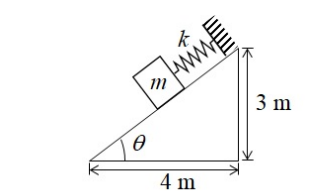
\includegraphics[width=\columnwidth]{question}
\end{center}
\end{figure}
\begin{enumerate}
    \item 30 N
    \item 45 N
    \item 60 N
    \item 75 N
\end{enumerate}
\hfill(GATE XE 2022)\\
\solution\\
\begin{table}[!ht] 
\centering
\setlength{\extrarowheight}{8pt}
\begin{tabular}{|l|l|l|}
    \hline
    \textbf{Parameter} & \textbf{Description} & \textbf{Value} \\
    \hline
     m & Mass of object & 10 Kg \\\hline
     $\mu$ & Frictional coefficient \brak{static} & 0.25\\\hline
     x\brak{t} & Displacement of block &  \\\hline
     $x\brak{0}$ & Initial displacement & 0 \brak{assumed} \\\hline
     g & Gravitational acceleration & 10 $m/s^2$ \\\hline
     $F_s$ & Spring force &  \\\hline
     f & frictional force &  $\mu$ N \\\hline
     N & Normal Force & mg $cos\brak{\theta}$ \\\hline
    \end{tabular}
  \vspace{4mm}
 \caption{Parameter Table}
 \label{tab:table0_xe80}
\end{table}

If the spring force is imum, frictional force is downwards and block is just about to move upwards and is at rest and equilibrium currently.\\
\begin{figure}[!ht]
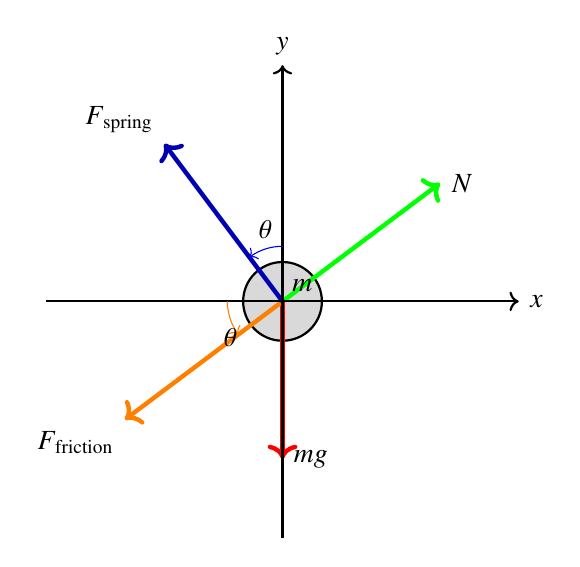
\begin{tikzpicture}
    \centering
    \draw[thick, fill=gray!30] (0,0) circle (0.5cm);
    
    \draw[->, ultra thick, green] (0,0) -- (2,1.5) node[right, black]{$N$};
    \draw[->, ultra thick, red] (0,0) -- (0,-2) node[right, black]{$mg$};
    \draw[->, ultra thick, orange] (0,0) -- (-2,-1.5) node[below left, black]{$F_{\text{friction}}$};
    \draw[->, ultra thick, blue!70!black] (0,0) -- (-1.5,2) node[above left, black]{$F_{\text{spring}}$};    
    
    \node at (0,0) [above right]{$m$};
    
    \draw[->, thick] (-3,0) -- (3,0) node[right]{$x$};
    \draw[->, thick] (0,-3) -- (0,3) node[above]{$y$};
    
    %approximated the angle to 37 degrees theta = 37 deg
    \draw[->, blue] (0,0) ++(90:0.7cm) arc (90:127:0.7cm) node[midway, above, black] {$\theta$};
    \draw[->, orange] (0,0) ++(180:0.7cm) arc (180:217:0.7cm) node[midway, below, black] {$\theta$};
\end{tikzpicture}
\caption{Maximum spring force FBD}
    \label{fig:fig1_xe80}
\end{figure}

From \figref{fig:fig1_xe80} and \tabref{tab:table0_xe80}, the force equation for the object is 
\begin{align}
    \mu mg \cos{\theta} + mg \sin{\theta} - F_{s} = m \frac{d^2x}{dt^2} \label{eq:eq1_xe80}
\end{align}
the Laplace transform of terms is 
\begin{align}
    k & \system{\mathcal{L}} \frac{k}{s}\\
    \frac{d^2x}{dt^2} & \system{\mathcal{L}} s^2 X\brak{s} - sx\brak{0} - \dot{x}\brak{0}
\end{align}
Applying Laplace transform to equation \eqref{eq:eq1_xe80},
\begin{align}
    \frac{ \mu mg \cos{\theta} + mg \sin{\theta} - F_{s}}{s} &= s^2 X\brak{s} - sx\brak{0} - \dot{x}\brak{0}\\
    \implies \frac{ \mu mg \cos{\theta} + mg \sin{\theta} - F_{s}}{s^3} &= X\brak{s} \label{eq:eq2_xe80}
\end{align}
The inverse Laplace transform is 
\begin{align}
     \frac{k}{s^3} \system{\mathcal{L^{ -}}} \frac{k}{2} t^2
\end{align}
The inverse Laplace of \eqref{eq:eq2_xe80} is
\begin{align}
    \brak{\mu mg \cos{\theta} + mg \sin{\theta} - F_{s}} t^2 = x\brak{t}
\end{align}
As it is always at equilibrium, $\frac{dx}{dt}$ is 0\\
\begin{align}
    2t \brak{\mu mg \cos{\theta} + mg \sin{\theta} - F_{s}} &= 0\\
    \implies \mu mg \cos{\theta} + mg \sin{\theta} - F_{s} &= 0\\
    \implies \mu mg \cos{\theta} + mg \sin{\theta} &= F_{s}
\end{align}
Using \tabref{tab:table0_xe80} , the maximum value for equilibrium is 
\begin{align}
    F_s = 80 N 
\end{align}
Now consider the other case. $F_s$ is minimum possible for equilibrium. The block is about to move downwards.\\
\begin{figure}[!ht]
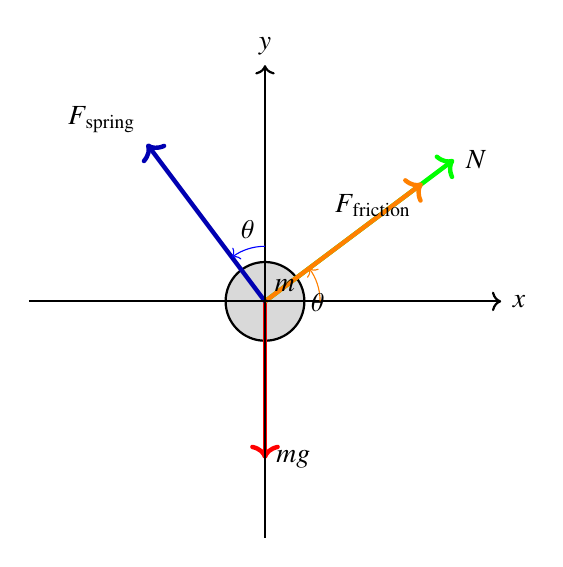
\begin{tikzpicture}
    \centering
    \draw[thick, fill=gray!30] (0,0) circle (0.5cm);
    
    \draw[->, ultra thick, green] (0,0) -- (2.4,1.8) node[right, black]{$N$};
    \draw[->, ultra thick, red] (0,0) -- (0,-2) node[right, black]{$mg$};
    \draw[->, ultra thick, orange] (0,0) -- (2,1.5) node[below left, black]{$F_{\text{friction}}$};
    \draw[->, ultra thick, blue!70!black] (0,0) -- (-1.5,2) node[above left, black]{$F_{\text{spring}}$};    
    
    \node at (0,0) [above right]{$m$};
    
    \draw[->, thick] (-3,0) -- (3,0) node[right]{$x$};
    \draw[->, thick] (0,-3) -- (0,3) node[above]{$y$};
    %approximated the angle to 37 degrees theta = 37 deg
    \draw[->, blue] (0,0) ++(90:0.7cm) arc (90:127:0.7cm) node[midway, above, black] {$\theta$};
    \draw[->, orange] (0,0) ++(0:0.7cm) arc (0:37:0.7cm) node[midway, below, black] {$\theta$};
\end{tikzpicture}
\caption{Minimum spring force FBD}
    \label{fig:fig2_xe80}
\end{figure}

From \figref{fig:fig2_xe80} and \tabref{tab:table0_xe80}, the force equation for the object is 
\begin{align}
     mg \sin{\theta} -\mu mg \cos{\theta} - F_{s} = m \frac{d^2x}{dt^2} \label{eq:eq3_xe80}
\end{align}
Laplace transform is 
\begin{align}
     \frac{ mg \sin{\theta} - \mu mg \cos{\theta} - F_{s}}{s^3} &= X\brak{s}
\end{align}
The inverse Laplace of \eqref{eq:eq2_xe80} is
\begin{align}
    \brak{ mg \sin{\theta} -\mu mg \cos{\theta} - F_{s}} t^2 = x\brak{t}
\end{align}
Hence the minimum force for equilibrium is
\begin{align}
    F_s &= mg \sin{\theta} - \mu mg \cos{\theta} \\
    &= 40 N
\end{align}
Hence , block is in equilibrium for $F_s$ between 40 and 80N. At 30 N, it is not at equilibrium.
\end{document}
